\documentclass{article}
\usepackage[utf8]{inputenc}
\usepackage{graphicx}

\title{Antworten zu Aufgabenblatt 1}
\date{2019-06-04}
\author{Alexander Lüngen}

\begin{document}
    \maketitle
    \newpage
    \section{Aufgabe 1}
        \subsection{a)}
        Die Reihenfolge in welcher die IDs der Threads ausgegeben werden ist jedes Mal unterschiedlich und ist auch nicht vorherzusagen.
        
        \subsection{b)}
        Gemessen wurde auf dem i82sn02. Für die manuelle Parallelisierung wurde atomic verwendet. Diese Messung wurde nach 4 Threads aufgehört da sich die Rechenzeit stark erhöht hat. Für das Parallelisieren mit Reduktion ist das maximales Speedup $ \sim 8 $.\\
        Bei 16 und 32 Threads verschlechtert sich die Beschleunigung im Gegensatz zu 8 Threads bei kleineren N. Das könnte am Overhead der Verarbeitung der Threads liegen.
        
	\begin{tabular}{|l|l|r|r|r|}
		\hline
		- & Number of Threads & N & Time (s) & Speedup \\
		\hline
		sequential & 1 & 1000 & 0.002 & - \\
		& 1 & $10^{7}$ & 0.239 & - \\
		& 1 & $10^{8}$ & 2.388 & - \\
		& 1 & $10^{9}$ & 23.642 & - \\
		& 1 & $10^{10}$ & 239.508 & - \\
		\hline
		manual & 2 & 1000 & 0.002 & 1 \\
		 & 2 & $10^{7}$ & 0.634 & - \\
		 & 2 & $10^{8}$ & 6.461 & - \\
		 & 2 & $10^{9}$ & 52.989 & - \\
		 & 4 & $10$ & 0.003 & - \\
		 & 4 & $10^{7}$ & 1.214 & - \\
		 & 4 & $10^{8}$ & 13.491 & - \\
		 & 4 & $10^{9}$ & $\sim$ 120 & - \\
		\hline
		reduction & 2 & 1000 & 0.002 & 1 \\
		 & 2 & $10^{7}$ & 0.121 & 1.9 \\
		 & 2 & $10^{8}$ & 1.188 & 2 \\
		 & 2 & $10^{9}$ & 11.845 & 1.9 \\
		 & 2 & $10^{10}$ & 118.204 & 2 \\
		 & 4 & 1000 & 0.003 & - \\
		 & 4 & $10^{7}$ & 0.062 & 3.9 \\
		 & 4 & $10^{8}$ & 0.595 & 4 \\
		 & 4 & $10^{9}$ & 5.959 & 3.9 \\
		 & 4 & $10^{10}$ & 59.183 & 4 \\
		 & 8 & 1000 & 0.003 & - \\
		 & 8 & $ 10^{7} $ & 0.032 & 7.5 \\
		 & 8 & $ 10^{8} $ & 0.299 & 7.9 \\
		 & 8 & $ 10^{9} $ & 2.967 & 7.9 \\
		 & 8 & $10^{10}$ & 29.689 & 8.0 \\
		 & 16 & 1000 & 0.003 & - \\
		 & 16 & $ 10^{7} $ & 0.040 & 5.9 \\
		 & 16 & $ 10^{8} $ & 0.318 & 7.5 \\
		 & 16 & $ 10^{9} $ & 3.028 & 7,8 \\
		 & 16 & $10^{10}$ & 29.674 & 8.1\\
		 & 32 & 1000 & 0.004 & - \\
		 & 32 & $ 10^{7} $ & 0.037 & 6.4 \\
		 & 32 & $ 10^{8} $ & 0.305 & 7,8 \\
		 & 32 & $ 10^{9} $ & 2.987 & 7.9 \\
		 & 32 & $10^{10}$ & 29.551 & 8.1 \\
		\hline
	\end{tabular}

	\newpage
        \subsection{c)}
        
        Die Messbedingungen waren gleich wie im Aufgabenteil b). Die Werte für das Speedup unterscheiden sich nicht groß von den oben gemessenen.\\
        
        \begin{tabular}{|l|r|r|r|}
        	\hline
        	 Auflösung N & No. Threads &  Time (s) & Speedup \\
        	 	\hline
        	 1000& 1 &  4.411 & - \\
        	 1000& 2 &  2.228 & 1.980 \\
        	 1000& 4 &  1.122 & 3.931 \\
        	 1000& 8 &  0.563 & 7.835\\
        	 1000& 16 &  0.567 & 7.780 \\
        	\hline
        	2000& 1 & 17.625 & - \\
        	2000& 2 &  8.896& 1.981 \\
        	2000& 4 &  4.493& 3.923 \\
        	2000& 8 &  2.254& 7.819 \\
        	2000& 16 &  2.248& 7.840 \\
        	\hline
        	4000& 1 & 71.761 & - \\
        	4000& 2 &  35.559 & 2.010 \\
        	4000& 4 &  17.952& 3.997 \\
        	4000& 8 &  8.978 & 7.991\\
        	4000& 16 &  8.980 & 7.991 \\
        	\hline
        	5000& 1 &  110.143 & - \\
        	5000& 2 &  55.564 & 1.982 \\
        	5000& 4 &  27.951 & 3.94 \\
        	5000& 8 &  13.995 & 7.870 \\
        	5000& 16 &  14.020 & 7.856\\
        	\hline
        \end{tabular}
	\begin{center}
		
\includegraphics[width=0.6\linewidth]{Aufgaben-Ressourcen/normal-1000.jpg}	
	\end{center}

	\begin{center}
		
\includegraphics[width=0.4\linewidth]{Aufgaben-Ressourcen/critical-1000.jpg}\quad
\includegraphics[width=0.4\linewidth]{Aufgaben-Ressourcen/critical-1000-1000.jpg}
		\\[\baselineskip]
		\includegraphics[width=0.4\linewidth]{Aufgaben-Ressourcen/critical-10000-1000.jpg}\quad\includegraphics[width=0.4\linewidth]{Aufgaben-Ressourcen/critical-10000-1000.jpg}
	\end{center}


    \section{Aufgabe 2}
    	\subsection{a)}
		\begin{enumerate}
			\item Example: Es besteht eine Race-Condition auf dem Array a über Index i,
				bei ungünstiger Ausführungsreihenfolge der Threads kann es dazu kommen,
				das a[i] durch einen Thread geschrieben wird und von einem anderen Thread versucht wird, darauf in der nachfolgenden Anweisung lesend zuzugreifen.
				Um dieses Problem zu lösen können zwei for-Schleifen verwendet werden.
				Eine schreibt alle Werte in Array a und die zweite schreibt alle Werte unter Zugriff auf Array a in Array b. 
				Beide Schleifen werden jeweils getrennt parallelisiert.
			\item Example: Threads exisiteren hier in der gesamten parallelen Region.
				Das nowait-Statement der ersten parallelisierten For-Schleife bewirkt, dass Threads bereits die nächste parallelisierte Schleife bearbeiten können, wenn sie ihren Teil der ersten Schleife fertig verarbeitet haben.
				Dies führt zu einer Race-Condition auf das Array a mit Index i, ähnlich zu Example 1.
				Mit dem entfernen des nowait-Statements der ersten for-Schleife warten alle Threads wieder auf die implizite Barriere bis alle Threads fertig sind und es kann Problemlos auf die geschriebenen Werte in Array a zugegriffen werden.
			\item Example: Hier ist die Variable x zunächst global definiert und wird somit implizit zwischen den Threads geshared. 
				Somit besteht eine Race-Condition auf x da die Threads unabhängig voneinander sowohl lesend als auch schreibend auf x zugreifen.
				Indem man x explizit als private deklariert, erhält jeder Thread seine eigene Kopie der Variable und es besteht keine Race-Condition mehr.
			\item Example: f ist global definiert und wird durch jeden Thread private gesetzt. 
				Allerdings erhält jeder Thread eine uninitialiserte Kopie der Variable f, was bedeutet das dass initialisieren mit dem Wert 2 vor der Schleife nur für den Master-Thread sichtbar ist.
				Um diese Initialiserung auch für alle übrigen Threads sichtbar zu machen, ist es erforderlich, f mittels firstprivate zu deklarieren.
				Des weiteren wird der Wert von x nicht aus der parallelen Region wieder rausgeschrieben, sondern gelöscht. 
				Wodurch der zuletzt geschriebene Wert innerhalb der parallelen Region in x nach außen hin nicht sichtbar ist.
				Um deses Verhalten zu erreichen, muss x als lastprivate deklariert werden.
			\item Example:

		\end{enumerate}

	\subsection{b)}

    \section{Aufgabe 3}
    
        \subsection{a)}
        P(x): Anzahl auszuführender Operationen auf x Prozessoren.\\
        T(x): Ausführungszeit auf x Prozessoren.\\
        
        \textbf{Speedup}:  $S(n) = T(1)/T(n) $. \\ Der Zusammenhang zwischen serieller und paralleler Ausführungszeit eines Programmes. Der Wertebereich ist $ 1 \leq S(n) \leq n $ .\\
        
        \textbf{Effizienz}: Die Effizienz $ E(n) = S(n)/n $ gibt die relative Verbesserung der Verarbeitungsgeschwindigkeit an.\\
        
        \textbf{Auslastung}: $ R(n)/(n*T(n)) $. Gibt an, wie viele Operationen (Tasks) jeder Prozessor im Durchschnitt pro Zeiteinheit ausgeführt hat.\\
        
        \textbf{Mehraufwand}: $ R(n) = P(n)/P(1) $. Beschreibt den bei einem Multiprozessorsystem erforderlichen Mehraufwand für die Organisation, Synchronisation und Kommunikation der Prozessoren.\\
        
        \subsection{b)}
        Race-Conditions: Wenn zwei Threads unabhängig voneinander auf eine Ressource lesend oder auch schreibend zugreiffen können, 
        spricht man von einer Race-Condition. Hierbei kann es bspw. beim Zugriff auf Variablen bei ungünstiger Ausführungszeiten
        dazu kommen, dass am Ende der Berechnungen ein falscher Wert in der Variable enthalten ist, als wenn die Berechnung sequentiell 
        ausgeführt worden wäre.
        Um eine Race-Condition zu vermeiden, können die kritischen Abschnitte in der Art und weise gesichert werden, das immer nur ein 
        Thread gleichzeitig innerhalb des kritischen Abschnitts sein darf.

        In diesem Zusammenhang kann es auch zu Deadlocks, Lifelocks oder auch Starvation kommen. 
        \subsection{c)}
        \begin{tabular}{|p{4cm}|p{3cm}|p{3cm}|p{3cm}|}
        	\hline
        	- & GPUs & CPUs & FPGAs \\
        	\hline
        	Energieeffizienz & Gut & Mittel & Gut  \\
        	\hline
        	Anwenderfreundlichkeit & \begin{itemize}
        		\item Braucht Einarbeitungszeit.
        		\item Es gibt Bibliotheken.
        	\end{itemize} & 
        \begin{itemize}
        	\item Am einfachsten zu programmieren.
        	\item Viele Bibliotheken vorhanden. 
        	\item Kurze Compilierzeit.
        \end{itemize}  & \begin{itemize}
        \item Aufwändig zu programmieren.
        \item Lange Compilierzeit.
        \item Wenig Bibliotheken.
    \end{itemize}  \\
        	\hline
        \end{tabular}\\
    
    In diesem Praktikum verwenden wir CPUs und GPUs da sie universeller einsetzbar sind als FPGAs und die Programmierung deutlich leichter ist.

    \section{Aufgabe 4}

    \section{Aufgabe 5}
	\subsection{a)}
	f(x,y) muss definiert sein auf $\Omega$ \newline
	$\Gamma$ ist der Rand von $\Omega$  \newline
	L\"{o}sung u(x,y) muss zweifach differenzierbar sein 
	\subsection{b)}
	f(x,y) = ($N^2$ + $M^2$)*4*$\pi^2$*sin(2*M*$\pi$*x)*sin(2*N*$\pi$*y)
	\subsection{c)}
	Es handelt sich um eine h-FEM.  \newline
	Die Lösungswerte in Figure \ref{A5L5}, \ref{A5L6} und \ref{A5L7} ergrben sich mit M=3; N=2; l=5,6,7;  \newline
	\begin{figure}
		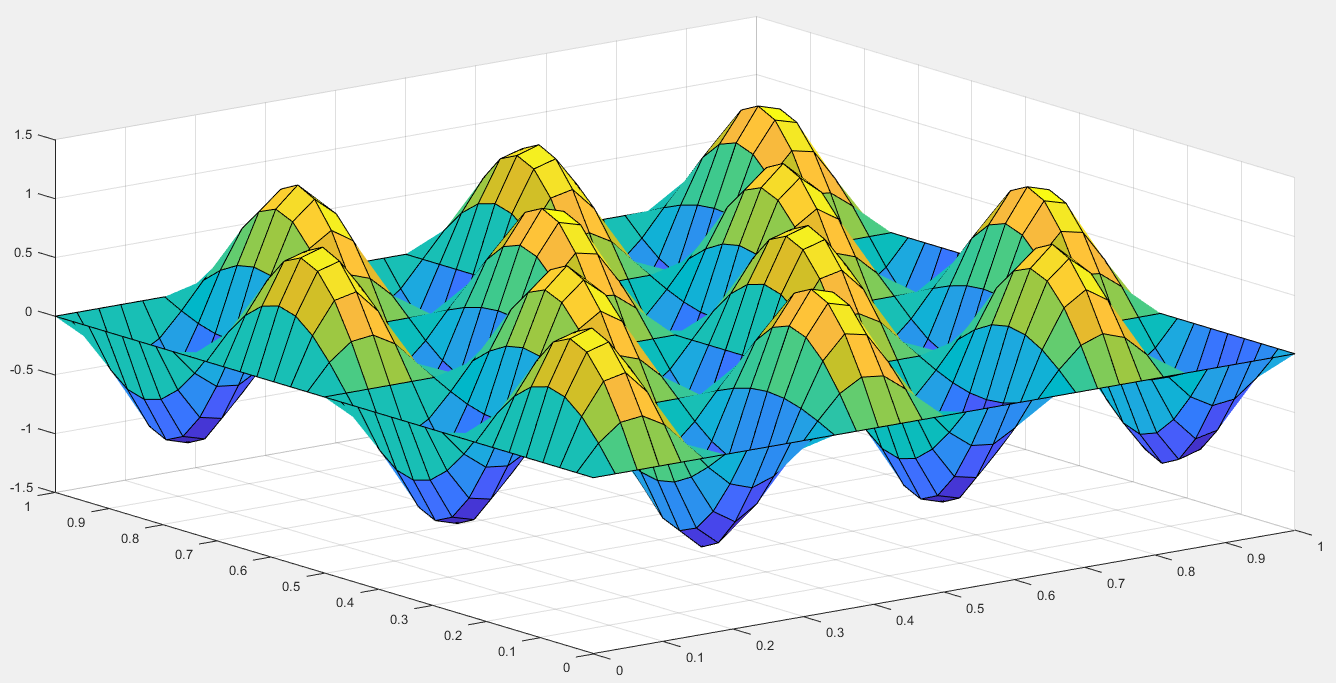
\includegraphics[width=\linewidth]{Aufgaben-Ressourcen/A5L5M3N2.png} 
		\caption{l=5; h=1/32;}
		\label{A5L5}
	\end{figure}
	\begin{figure}
		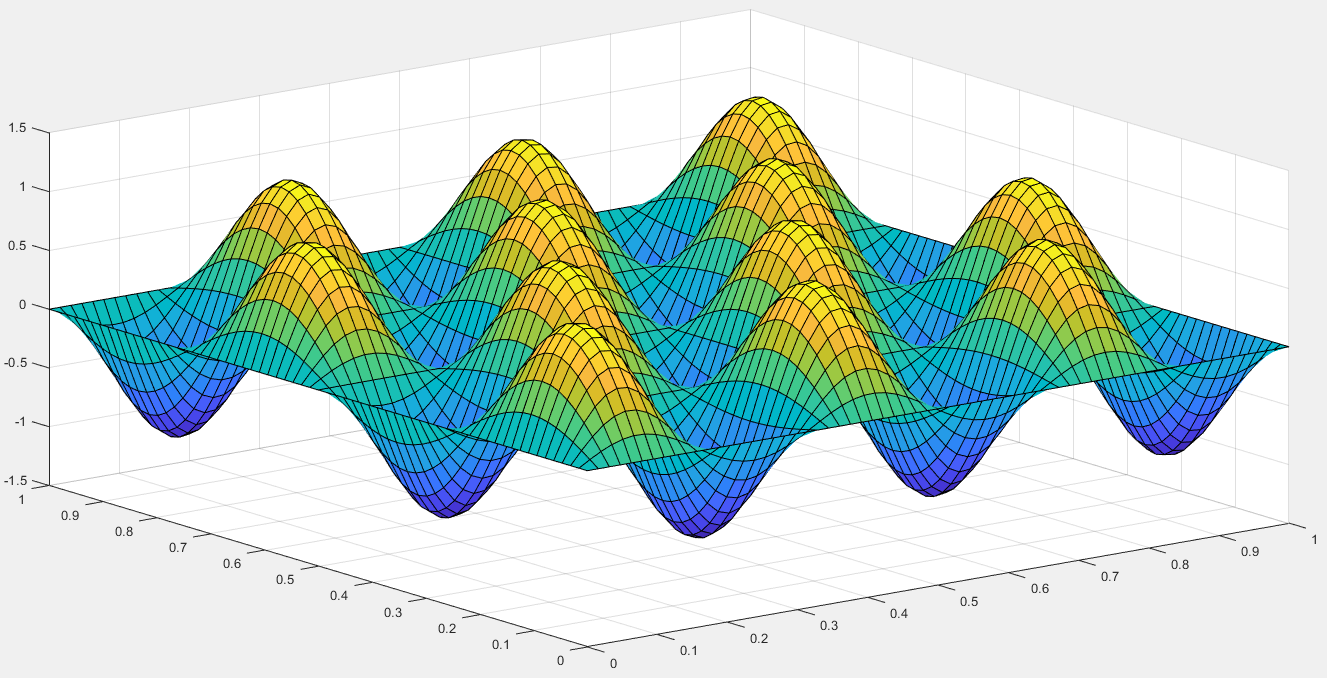
\includegraphics[width=\linewidth]{Aufgaben-Ressourcen/A5L6M3N2.png} 
		\caption{l=6; h=1/64;}
		\label{A5L6}
	\end{figure}
	\begin{figure}
		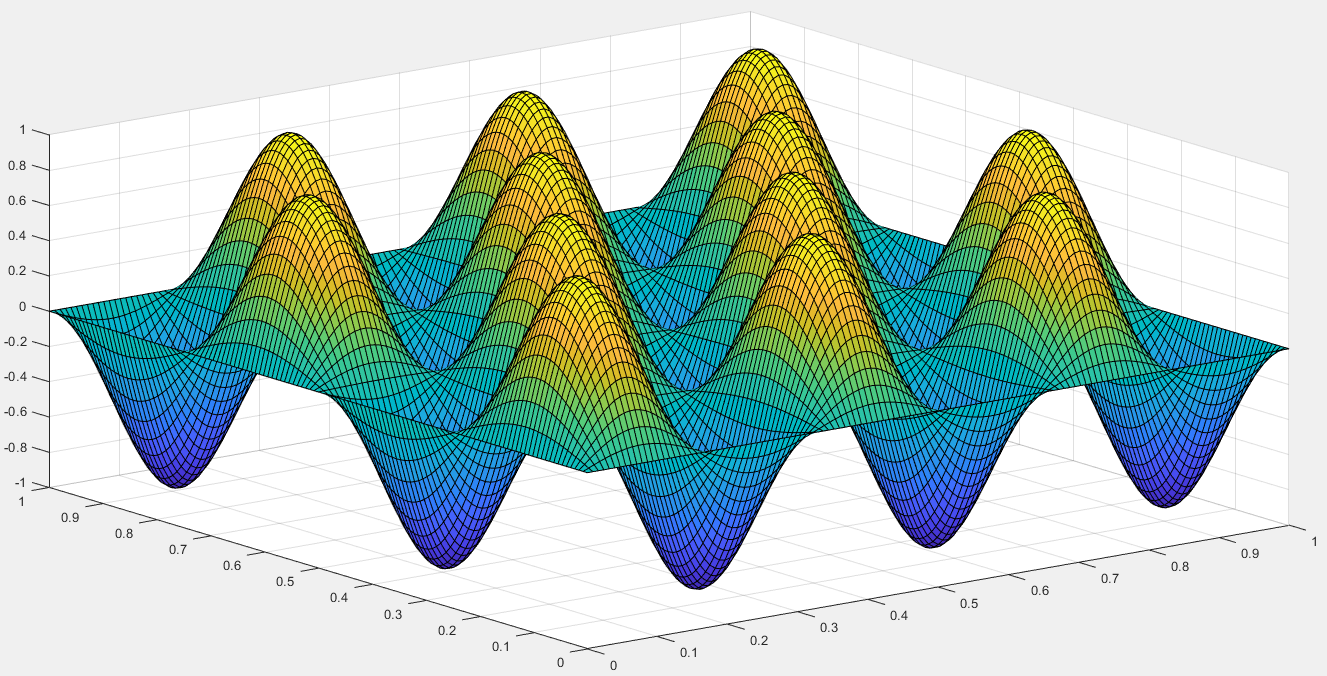
\includegraphics[width=\linewidth]{Aufgaben-Ressourcen/A5L7M3N2.png}
		\caption{l=7; h=1/128;}
		\label{A5L7}
	\end{figure}

\section{Aufgabe 6}
	\subsection{a)}
	Liste: CG Verfahren; PCG-Verfahren; Verfahren der minimalen Risiduen(GMRES); GCR-Verfahren; Arnoldi-Verfahren; FOM, ORTHORES;\newline
	Das Gleichungssystem ist dünnbesetzt zbd alle Krylow-Unterraumverfahren sind gut geeignet für dünnvesetzte Gleichungssysteme.
	Diese Lösungswerte in Figure \ref{A6L5}, \ref{A6L6} und \ref{A6L7} ergeben sich mit der Gleichung aus Aufgabe 5 und M=3; N=2; l=5,6,7;  \newline
\begin{figure}
	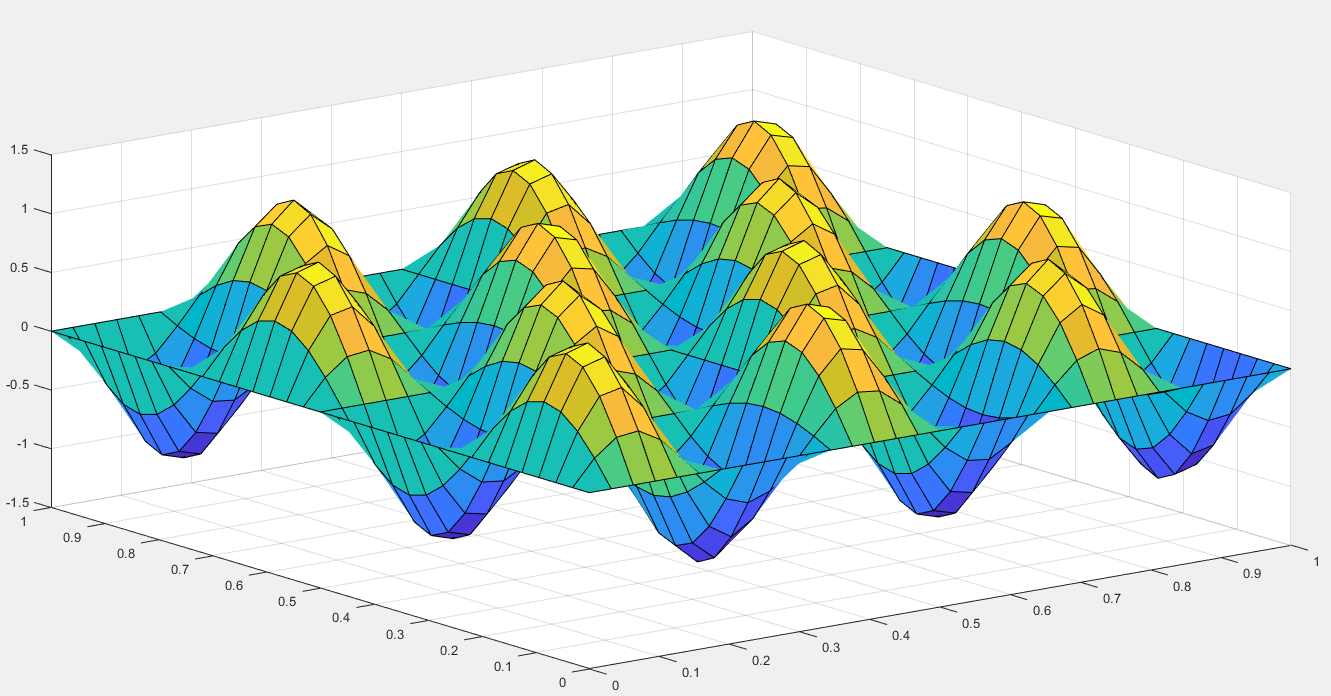
\includegraphics[width=\linewidth]{Aufgaben-Ressourcen/A6L5M3N2.png} 
		\caption{GMRES; l=5; h=1/32;}
		\label{A6L5}
\end{figure}
\begin{figure}
	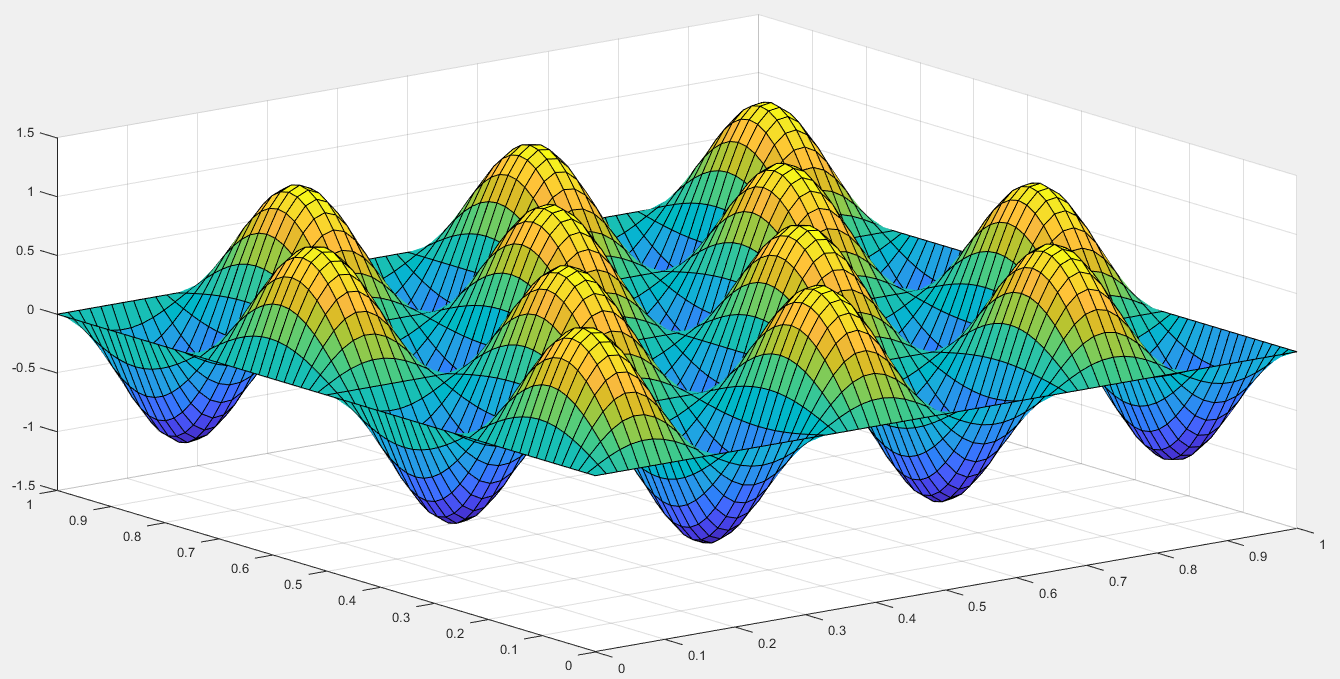
\includegraphics[width=\linewidth]{Aufgaben-Ressourcen/A6L6M3N2.png} 
		\caption{GMRES; l=6; h=1/64;}
		\label{A6L6}
\end{figure}
\begin{figure}
	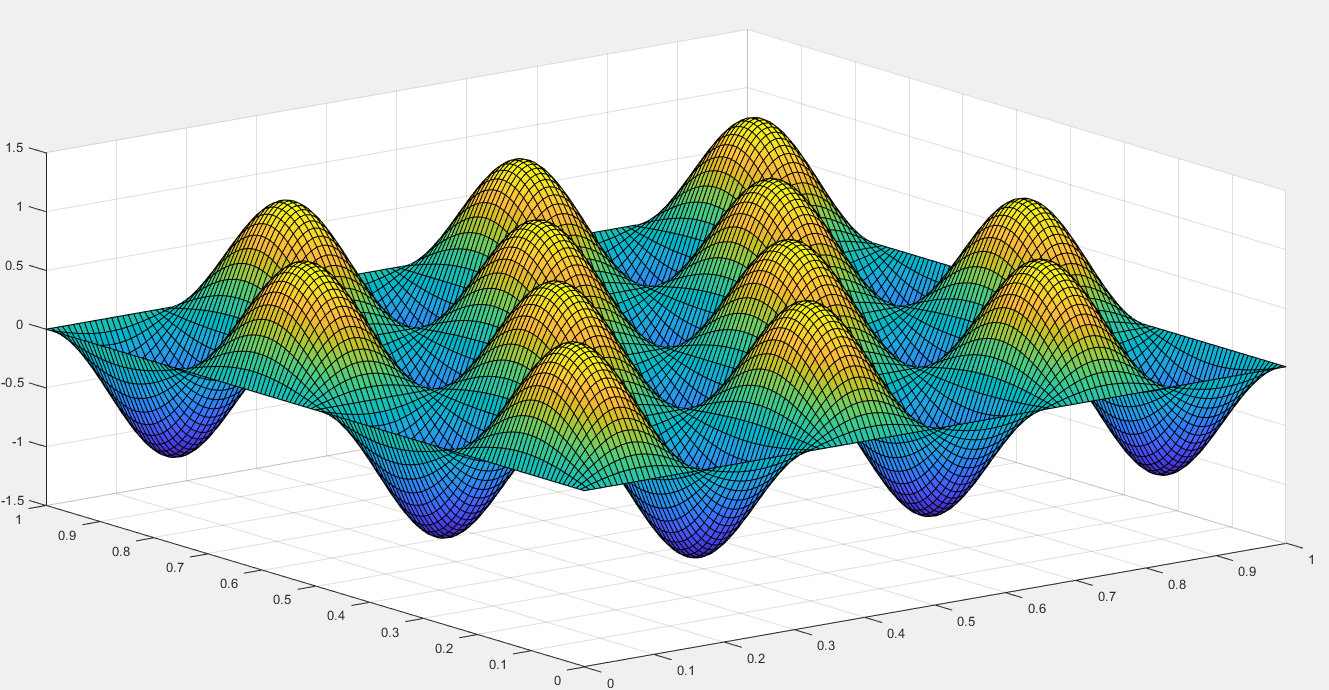
\includegraphics[width=\linewidth]{Aufgaben-Ressourcen/A6L7M3N2.png}
		\caption{GMRES; l=7; h=1/128;}
		\label{A6L7}
\end{figure}
	\subsection{b)}
	Die Verwendung des Residuums als Abrruchbedingung ist eventuell problematisch, da man dadurch in jedem Schleifendurchlauf einen Lösungsvektor $x^k$ berechnen muss. Man kann sich eine feste Anzahl von Iterationen setzen, allerdings hat man dann keine garantierte Genauigkeit. Außerdem kann man das Residuum mit weniger Rechenaufwand in jeder Iteration abschätzen und diesen Schätzwert als Abbruchbedingung nutzen. Auch diese Vorgehensweise hat keine garantierte Genauigkeit, da die Schätzgenauigkeit variiert.
	\subsection{c)}

Einsatz eines Vorkonditionierers: Der Einsatz ist unsinnvoll, da wir bereits eine dünn besetzte Matrix gegeben haben. Falls die Matrix anders besetzt wäre, könnte ein Vorkonditionierer von Nutzen sein.
	\subsection{d)}
\section{Aufgabe 7}
\end{document}
